\chapter{System}
The software that is used in the autonomous landing system is based on the LSTS toolchain \citep{pinto2013lsts}, with \gls{rtk-gps} solution calculated in RTKLib. The toolchain was developed for support of networked heterogeneous air and ocean vehicle systems. The toolchain supports interactions over wireless network, and is supports interaction with different system responseable for the low end control. The toolchain contain four different modules, namely \gls{imc}, DUNE, NEPTUS and Glued.
\section{Navigation system}
The navigation system receive state information mainly from the pixhawk, however the the system is able to receive position and velocity from a \gls{rtk-gps} subsystem were the solution is calculated in RTKLib. The system decide if it should use \gls{rtk-gps} through a DUNE task which manage the the source of the navigation data, which will be referred to as the navigation task.

The operator can monitor which source is used in the navigation task through a interface that indicate which source is available.

\subsection{RTK-GPS system}
The navigation system receive its \gls{rtk-gps} solution from a DUNE task, which is connected to the open-source program RTKLib \citep{takasu2009development}. RTKLib contains several separated program that can be used in the field of \gls{rtk-gps}, where the program rtkrcv is used in the \gls{uav} to calculate the \gls{rtk-gps} solution. The program that is used in the base station is str2str, which retrieve the raw data from a GNSS receiver and transmits the data over tcp to the \gls{uav}. The GPS receivers that is used in both the \gls{uav} and base station is a Ublox Lea M8T. The structure of the RTKLib software configured with a rover and base station is shown in figure \ref{figure:RTKLIB_STRUCTURE}

\begin{figure}[H]
	\centering
		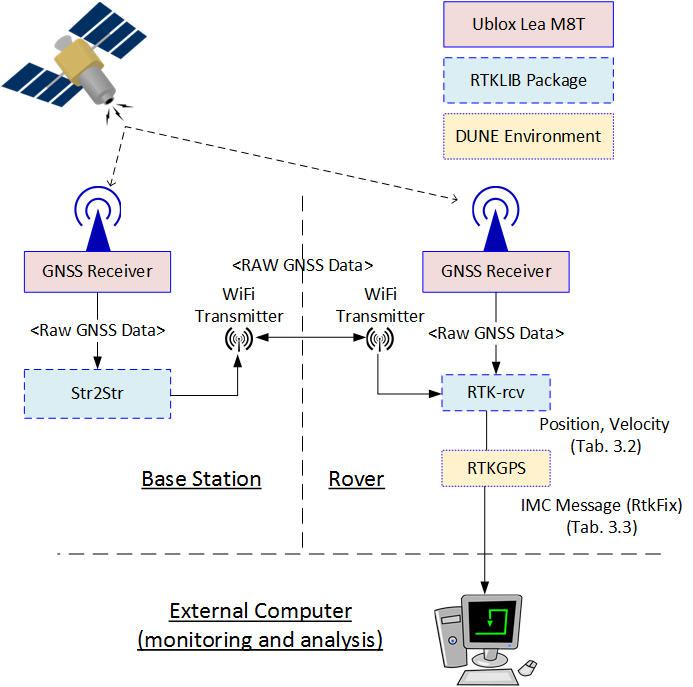
\includegraphics[width=1\textwidth]{figs/RTKLIB.png}
		\caption{The communication structure of \gls{rtklib}}
		\label{figure:RTKLIB_STRUCTURE}
\end{figure}
As part of the \gls{rtk-gps} system the base station has it's own DUNE task running that calculate the position of the base station. The operator has to decide when the the \gls{gps} position of the base station should be considered as fixed, which will result in that the \gls{rtk-gps} DUNE task can include the base station in it's \gls{imc} message. This is require since RTKLib does not include the base position in it's output message. 
\subsection{Navigation source}
The source of the position and velocity solution which is the output from the navigation system is decided in a DUNE task that consume both sensor data from the \gls{rtk-gps} system and the pixhawk. A requirement for use of \gls{rtk-gps} is that the position of the base station is fixed and included in the \gls{imc} message from the \gls{rtk-gps} task, in addition that the operator has decided that \gls{rtk-gps} should be used if available and the \gls{rtk-gps} solution is fixed.

The navigation allows for use of float solution of \gls{rtk-gps} given that it has previous been fixed, for a limited time. 

\subsection{Operator interface}
A interface for navigation source monitoring has been created in Neptus in order to ease monitoring of which source the \gls{uav} is using as position and velocity source. The interfaced apply a color code to indicate which source is currently in use in addition to all sensor system that are available, as seen in table \ref{Tb:Color Code}.

\begin{table}[H]
\begin{center}
    \begin{tabular}{ | l | l |}
    \hline
    \textbf{Color} & \textbf{Description} \\ \hline
    White & Not available \\ \hline
    Yellow & Available, but not in use \\ \hline
    Green & Available, and in use \\ \hline
    \end{tabular}
\end{center}
\caption{Net approach parameters }
\label{Tb:Color Code}
\end{table}

%\subsection{Position correction}%Flytt til resultat
%The highly dynaimcal nature of the uav create a challenge for the navigation system due to the blocking of the gps antenna from the satellite constellation. The problem was reduced by using a gps receiver that has a high performance in satellite tracking, however this does not remove the problem. A float solution from the gps system is valid for some seconds after fix is lost, due to the predictive nature of the Extended Kalman filter in rtklib. However after a seartin amount of time the navigation system swithces over to use the position estimate from the pixhawk, which has a lower accuracy level then the rtk gps system. To increase the accuracy level a offset solution is proposed. By calculating the difference between the fixed rtk gps solution and the position solution from the pixhawk a offset can be found. If the offset can be assumed constant or quasi stationary it can be used to increase to accuracy level for the navigation system enough to allow for completion of critical phases of a manoeuvre. However tests showed that the offset was not constant nor quasi stationary. By applying the offset to the pixhawk position solution the accuracy level will increase, but not enough to allow for execution of critical manoeuvres.
%In order to make the navigation system more robust, some methods was explored. 
\section{Path generation}
The landing plan is design with the assumption that the aerial space in which the uav operates is limited. The limitation can be the range of the uav, regulatory limits or weather. In addition the autonomous landing system must be able to perform a safe landing from any initial position. Furthermore the size of the virtual run way should be constructed by the operator. The type of uav operation dictates the maximum size of the landing path. Different types of uav operation is LOS, ELOS, BLOS and BRLOS. Only the first is considered in this thesis, which means that the pilot must have the uav in view during the entire flight. The operator must also be able to control the angle which the uav is descending, which means that the height of the landing path is fixed. Therefore the uav must be at the correct altitude before it can start descending toward the landing net.

A landing plan that is proposed consist of Dubins path \ref{S:DubinsPath} in the lateral plane, and straight lines in the longitudinal plane. The path is generated from an arbitrary start positing, and will create a continuous path toward the landing approach. The design is inspired by the work done in \citep{Skulstad&Syversen} were way-points was used to guide the uav toward the landing approach.

The plan is generated in a Dune task which receive a plan generation request from Neptus. Then a plan is created, which is sent to the Dune task Plan manager, which in turn sent desired state to the guidance system. The plan is decoupled from the guidance system, which allow for use of different control design when executing the landing plan.

The Dubin path is constructed with a followPath manoeuvre.

The landing plan generated by the Dune task can be requested for review by the operator in Neptus. The plan will not start before the operator has reviewed the plan, and approved by uploading it to the uav. In the uploaded version a specification list on which controller that should be used is included.  
\subsection{The net approach}
The net approach path consist a straight line in the lateral plain, and straight lines in the longitudinal plane. The net approach way-points are defined relative to the position of the net, which has been defined as origo. The four way-points in the net approach is defined as follows:
\begin{subequations}
\begin{align}
&\mathbf{WP1} = 
\begin{bmatrix}
-a0 \\
0 \\
h_{nc} + a1\tan(\gamma_a) 
\end{bmatrix}\\
&\mathbf{WP2} = 
\begin{bmatrix}
a1 \\
0 \\
h_{nc} - a1\tan(\gamma_a)
\end{bmatrix}\\
&\mathbf{WP3} = \mathbf{WP2} + 
\begin{bmatrix}
a2 \\
0 \\
a2\tan(\gamma_d)
\end{bmatrix}\\
&\mathbf{WP4} = \mathbf{WP3} + 
\begin{bmatrix}
a3 \\
0 \\
0 \\
\end{bmatrix}
\end{align}
\end{subequations}
were the description of the parameters used is given in table \ref{Tb:Approach Parameters}. The net is placed between the first and second way points such that transitional behaviour do not occur during the finale stage of the net landing. In addition the path has been made with the assumption that the $\gamma_a$ and $\gamma_d$ is considered small. This assumption is made to easy the demand of the controllers used in the landing system.
\begin{table}[H]
\begin{center}
    \begin{tabular}{ | l | l |}
    \hline
    \textbf{Parameter} & \textbf{Description} \\ \hline
    $a0$ & The distance behind the net \\ \hline
    $a1$ & The distance in front of the net \\ \hline
    $a2$ & The length of the glide slope \\ \hline
    $a3$ & The length of the approach towards the glide slope \\ \hline
    $\gamma_a$ & The net attack angle \\ \hline
    $\gamma_d$ & The glide slope angle \\ \hline
    \end{tabular}
\end{center}
\caption{Net approach parameters }
\label{Tb:Approach Parameters}
\end{table}
The way point vectors are rotated into the NED frame by a rotation around the z-axes.
\begin{equation}
WP^n = R(\psi_{net})WP^b
\end{equation}
were $\psi_{net}$ is the heading of the net.
\begin{figure}
\def\svgwidth{\textwidth} % Defining the width since Inkscape hasn't done this yet in the .pdf_tex file
\input{InkFig/LandingPhase.pdf_tex}
\end{figure}

\subsection{The landing path approach}
In order for the \gls{uav} to be able to start the landing approach the \gls{uav} must be at the correct altitude with the correct orientation from any initial position. That require a path which the \gls{uav} is able to follow. The problem can be separated into two parts. The first is the longitudinal parts, while the other is the lateral. The longitudinal path will be more exposed to large changes in heading, which puts demands of the type of path that can be chosen. However since a time demand is not required the problem becomes a path following problem. The problem has been solved by creating a Dubins path in the longitudinal plane.

A desired behaviour in the lateral plane is that the \gls{uav} should have a controlled decent. Given this desired behaviour it was decided that the lateral plane should be a glide slope, which means that the decent angle can be considered small. The strategy chosen to solve this problem is the use of straight lines in the lateral plane. The straight lines are is included with Dubins path such that the turn in Dubins path becomes a spiral.

At the end of Dubins path the path is checked if the correct height has been reach. If the correct height has not been reached the path will create a spiral that converge to the correct height. When the correct height has been reach a last arc is created in order for the \gls{uav} to get the correct orientation.

The landing path can be created in two modes, which is manual or automatic. The manual mode allow the operator to design the landing path by defined the turning direction for the start and final circle. This enable the operator to specify a path that fills a operational demand, which would not necessary be the path when in automatic.

In automatic mode all four variants, which is given in table \ref{Tb:DubinsTurningDirection}, calculated. After the length of the paths are calculated, where the shortest path is chosen to be the landing path.
The landing path approach can be generated in to different way. One mode allow for manual deciding which side the start and finish circle should be in respect on the start pose, and the net landing approach. This allow the operator full control over the landing path, and can choose a landing path that is operation feasible and not necessary the shortest path. 
\subsubsection{Extra way point}
To ensure that the path generation system will generate å flyable path an extra way point is added in the case of the start pose in cause an infeasable dubins path, or an spesial case of Dubins path which has not been implemented. The two case are
\begin{subequations}
\end{subequations}
\section{Evasion}
To ensure the safety of the operator a evasion controller is used to abort the landing when a successful landing is deemed infeasible or improbable.

\section{Guidance system}
The guidance system consist of two part. Sliding mode controller, and a los controller

\subsection{Sliding mode controller}
For course control the system use a sliding mode controller that was proposed in the paper \citep{fortuna2015cascaded}, which USGES stability property.
\begin{subequations}
\begin{align}
\dot{x} &= V_a\cos(\psi) + W_x = V_g\cos(\psi) \\
\dot{y} &= V_a\sin(\psi) + W_y = V_g\sin(\psi) \\
\dot{phi} &= \frac{g}{V_a}\tan(\varphi) \\
\dot{\varphi} &= -\frac{\varphi-\varphi_{cmd}}{T_\varphi} \\
W &= \sqrt{W_x^2 + W_y^2}
\end{align}
\end{subequations}
\begin{equation}
\epsilon(\varphi) = \begin{cases}
\cos(\varphi), & \text{if}\ |\cos(\varphi)|\geq\epsilon'\\
\epsilon', & \text{if}\ 0 \leq \cos(\varphi) < \epsilon' \\
-\epsilon', & \text{if} -\epsilon'<\cos(\varphi) < 0
\end{cases}
\end{equation}
\begin{equation}
\chi = \tan^{-1}(\frac{\dot{y}}{\dot{x}})
\end{equation}
\begin{equation}
\dot{\chi} = \frac{g\sin(\varphi)(V_a + \cos(\psi)W_x + \sin(\psi)W_y}{\epsilon(\varphi)V_g^2}
\end{equation}
\begin{subequations}
\begin{align}
\chi_d &= \tan^{-1}(-\frac{t}{\Delta} \\
\dot{\chi_d} &= -\frac{\Delta}{\Delta^2+y^2}\dot{y} \\
\ddot{\chi} &= \frac{\Delta}{(\Delta^2 + y^2)^2}(2y\dot{y}^2 - (\Delta^2 + y^2)\ddot{y})
\end{align}
\end{subequations}
\begin{equation}
\tilde{\chi} = \chi - \chi_d
\end{equation}
\begin{equation}
s = \dot{\tilde{\chi}} + \lambda\tilde{\chi}
\end{equation}
\begin{equation}
u = -\lambda\dot{\tilde{\chi}} - \rho\text{sgn}(s) - K_ds
\end{equation}